\section{Trabalhos Relacionados} \label{sec:trabrel}
Nesta seção, apresentar-se-ão exemplificações de projetos preexistentes que, até o momento, podem ou não ter sido concretizados na sociedade. Algumas das resoluções subsequentes implicam distintas metodologias, abrangendo desde a automatização das coberturas até a aplicação de Inteligência Artificial para a identificação de materiais por meio de sensores, permitindo, desse modo, a segregação dos resíduos com base em sua tipologia.


\cite{lisa} Lixeira Inteligente Seletiva Automática (LISA), entrega o projeto de uma lixeira inteligente que separa por materiais o lixo jogado nele. Os sensores são os responsáveis por detectar o material do lixo jogado e enviar informações via \textit{bluetooth} e a placa utilizada é o Arduino UNO.

 \begin{figure}[H]
    
    \label{fig:lisa}
    \begin{center}
        
        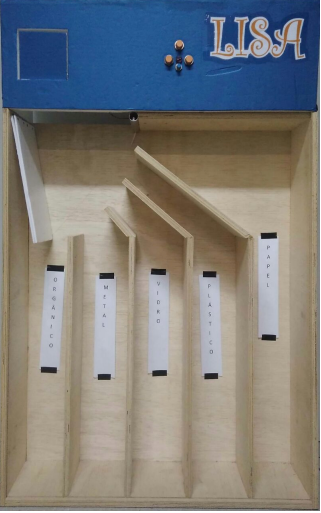
\includegraphics[scale=0.5]{Textuais/imagens/lisa.png}
        
        Fonte: \cite{lisa}
    \end{center}
\end{figure}

\cite{gaia}, o projeto GAIA apresenta a ideia de um robô inteligente que fará o trabalho de separar o lixo por categorias: plástico, vidro, papel e metal. Trata-se de um braço robô que possui uma câmera que detecta o \textit{ID} determinado por cada material e faz a separação necessária colocando o lixo em seu compartimento determinado.

 \begin{figure}[H]
    \label{fig:gaia}
    \begin{center}
        
        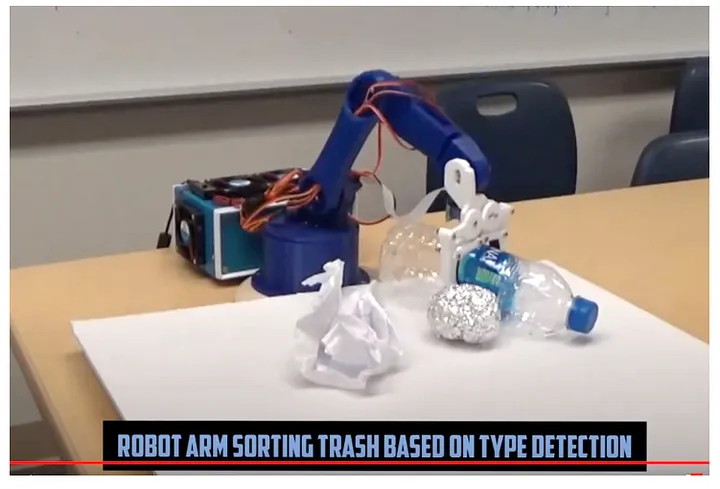
\includegraphics[scale=0.5]{Textuais/imagens/gaia.png}
        
        Fonte: \cite{gaia}
    \end{center}
\end{figure}

\cite{smartbin},  os principais locais onde o projeto pode ser instalado são os locais como shoppings, aeroportos, cinemas etc.  O projeto SmartBin é de fácil utilização e possui boa eficiência, existe a separação por 4 categorias, plástico, vidro, papel e metal. A tecnologia de espectroscopia infravermelha que é responsável pela classificação desses materiais.

 \begin{figure}[H]
    
    \label{fig:smartbin}
    \begin{center}
        
        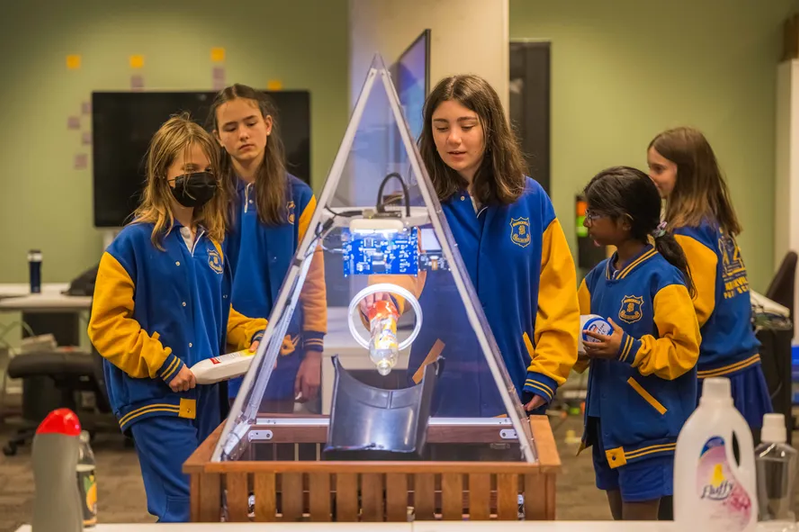
\includegraphics[scale=0.5]{Textuais/imagens/smart.png}
        
        Fonte: \cite{smartbin}
    \end{center}
\end{figure}



